Considerando l'architettura hardware precedente, è possibile, effettivamente, implementare un approccio più veloce dal punto di vista delle operazioni, cioè una soluzione basata su parallelismo. In particolare, allocando un maggior numero di risorse, è possibile eseguire delle operazioni in parallelo riducendo di conseguenza la latenza, cioè il tempo di esecuzione totale.
\\
Tale approccio è possibile implementarlo in due modi differenti:
\begin{itemize}
    \item \textbf{Manuale}\\Unrolling ottenuto tramite rimodulazione software
    \item \textbf{Automatico}\\Unrolling ottenuto tramite direttiva proprietaria (pragma)
\end{itemize}

In particolare, sia l'unrolling manuale sia quello automatico, sono stati ottenuti considerando sia un fattore di parallelismo pari a 2 sia pari a 4. Inoltre, bisogna specificare che, per quanto riguarda l'unrolling automatico (tramite pragma), è stata realizzata un'ulteriore soluzione hardware, tenendo conto sia del fattore 2 sia del fattore 4, dove è stato considerato sia il pragma di unrolling sia il pragma di partitioning. Il partizionamento serve per risolvere un problema tipicamente causato dagli array. Gli array sono implementati come BRAM, solitamente progettate per un dual-port massimo. Questo può limitare il throughput di un algoritmo ad alta intensità di read/write. La larghezza di banda può essere migliorata dividendo l'array (una singola BRAM) in array più piccoli (più BRAM), aumentando di fatto il numero di porte. Gli array vengono partizionati utilizzando la direttiva ARRAY\_PARTITION. Vivado HLS offre tre tipi di partizionamento degli array. I tre tipi di partizionamento sono:
\begin{itemize}
    \item \textbf{block}\\L'array originale viene suddiviso in blocchi di uguali dimensioni di elementi consecutivi dell'array originale.
    \item \textbf{cyclic}\\L'array originale viene suddiviso in blocchi di uguali dimensioni che interlacciano gli elementi dell'array originale.
    \item \textbf{complete}\\L'operazione predefinita consiste nel dividere l'array nei suoi singoli elementi. Ciò corrisponde alla risoluzione di una memoria in registri.
\end{itemize}

\begin{figure}[H]
    \centering
    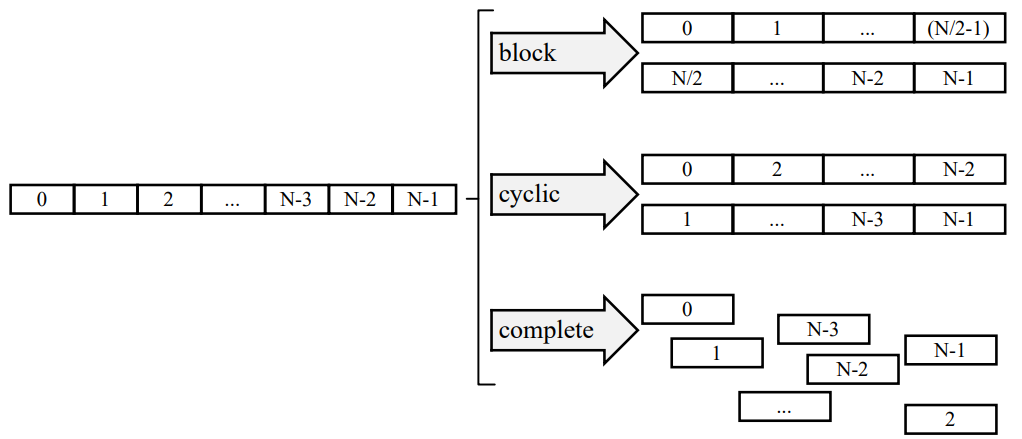
\includegraphics[width=1\textwidth]{solutions/loop_unrolling/partitioning.png}
    \caption{HLS Array Partitioning}
\end{figure}

Pertanto, è possibile elencare qui di seguito le soluzioni hardware progettate per l'approccio del parallelismo:
\begin{itemize}
    \item Unrolling Manuale Fattore=2
    \item Unrolling Manuale Fattore=4
    \item Unrolling Automatico Fattore=2
    \item Unrolling Automatico Fattore=4
    \item Unrolling Automatico con Partitioning Fattore=2
    \item Unrolling Automatico con Partitioning Fattore=4
\end{itemize}

\begin{figure}[H]
    \centering
    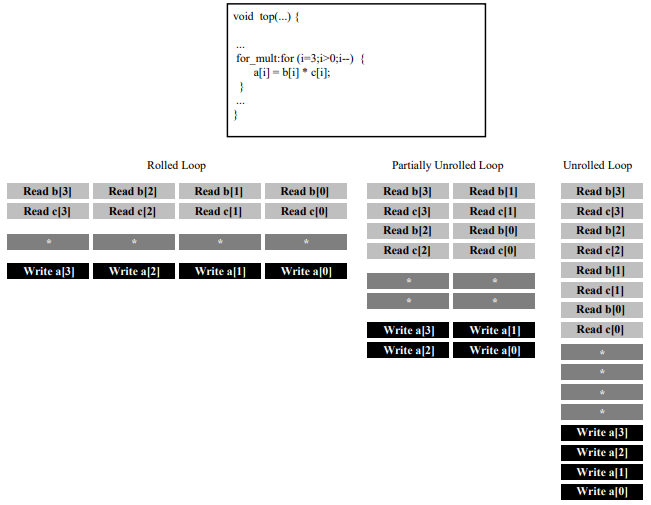
\includegraphics[width=1\textwidth]{solutions/loop_unrolling/unrolling.png}
    \caption{HLS Loop Unrolling}
\end{figure}

A questo proposito, verranno analizzati i report considerando le soluzioni hardware aventi stesso fattore così da poter effettuare confronti adeguati tra le varie implementazioni.In particolare, è stato considerato un loop unrolling di fattore 2 e un fattore 4. Ovviamente, la figura sopra allegata è solo un esempio per rappresentare meglio il concetto di unrolling e partitioning.

\subsubsection{Loop Unrolling Factor=2}
\lstinputlisting[language=C++]{solutions/loop_unrolling/factor2/fir_loop_unrolling_manual_factor2.cpp}
\lstinputlisting[language=C++]{solutions/loop_unrolling/factor2/fir_loop_unrolling_automatic_factor2.cpp}
\lstinputlisting[language=C++]{solutions/loop_unrolling/factor2/fir_loop_unrolling_automatic_partiotioning_factor2.cpp}

\begin{table}[H]
    \centering
    \begin{tabular}{|c|c|c|c|c|}
        \hline
        \textbf{Solution} & \textbf{Clock} & \textbf{Target} & \textbf{Estimated} & \textbf{Uncertainty} \\
        \hline
        Manuale & ap\_clk & 10.00 & 8.510 & 1.25 \\
        \hline
        Automatico & ap\_clk & 10.00 & 8.510 & 1.25 \\
        \hline
        Automatico con Partitioning & ap\_clk & 10.00 & 8.510 & 1.25 \\
        \hline
    \end{tabular}
    \caption{HLS Loop Unrolling Factor=2 Solution Timing Summary (ns)}
    \label{tab:hls-loop-unrolling-factor2-solution-timing-summary}
\end{table}

Si può notare come la latenza associata alla soluzione hardware basata su unrolling manuale sia la medesima di quella basata su unrolling automatico (effettuato mediante pragma). Questo è dovuto al fatto che l'implementazione è la stessa: nel primo caso è effettuato manualmente mentre nel secondo caso è effettuato mediante direttiva proprietaria del tool. Invece, nel caso della soluzione hardware basata su unrolling automatico e partitioning, si riscontra una latenza maggiore. Questo risultato è dovuto al fatto che, tramite il pragma di partizionamento, si è dovuto gestire, inoltre, letture e scritture in parallelo.

\begin{table}[H]
    \centering
    \begin{tabular}{|c|c|c|c|c|}
        \hline
        \multicolumn{1}{|c|}{\textbf{Solution}} & \multicolumn{2}{|c|}{\textbf{Latency}} & \multicolumn{2}{|c|}{\textbf{Interval}} \\
        & min & max & min & max \\
        \hline
        Manuale & 56 & 56 & 56 & 56 \\
        \hline
        Automatico & 56 & 56 & 56 & 56 \\
        \hline
        Automatico con Partitioning & 61 & 66 & 61 & 66 \\
        \hline
    \end{tabular}
    \caption{HLS Loop Unrolling Factor=2 Solution Latency Summary (clock cycles)}
    \label{tab:hls-loop-unrolling-factor2-solution-latency-summary}
\end{table}

Si può evidenziare come, nel caso della soluzione hardware con urolling automatico e partizionamento, l'aumento della latenza si ha soltanto in corrispondenza del loop di shifting, cioè proprio dove è stato collocato il pragma di partitioning.

\begin{table}[H]
    \centering
    \begin{tabular}{|c|c|c|c|c|c|c|c|c|c|}
        \hline
        \multicolumn{1}{|c|}{\textbf{Solution}} & \multicolumn{1}{|c|}{Loop Name} & \multicolumn{2}{|c|}{\textbf{Latency}} & \multicolumn{2}{c|}{\textbf{Iteration Latency}} & \multicolumn{2}{c|}{\textbf{Initiation Interval}} & \multicolumn{1}{c|}{\textbf{Trip}}  \\
        &  & min & max & min & max & achieved & target & \textbf{Count} \\
        \hline
        Manuale & - loopShifting & 10 & 10 & 2 & 2 & - & - & 5 \\
        & - loopAccumulator & 44 & 44 & 4 & 4 & - & - & 11 \\
        \hline
        Automatico & - loopShifting & 10 & 10 & 2 & 2 & - & - & 5 \\
        & - loopAccumulator & 44 & 44 & 4 & 4 & - & - & 11 \\
        \hline
        Automatico  & - loopShifting & 15 & 20 & 3 & 4 & - & - & 5 \\
        con Partitioning & - loopAccumulator & 44 & 44 & 4 & 4 & - & - & 11 \\
        \hline
    \end{tabular}
    \caption{HLS Loop Unrolling Factor=2 Solution Latency Loops Summary }
    \label{tab:hls-loop-unrolling-factor2-solution-loop-summary}
\end{table}

Aprendo la sezione Analysis del tool si può vedere meglio nel dettaglio che, all'interno del loop di shifting, sono presenti 2 shifting in parallelo (dal momento che è stato considerato un fattore di parallelismo pari a 2) sia peer la soluzione hardware di unrolling manuale sia per quella di unrolling automatico (mediante pragma).

\begin{figure}[H]
    \centering
    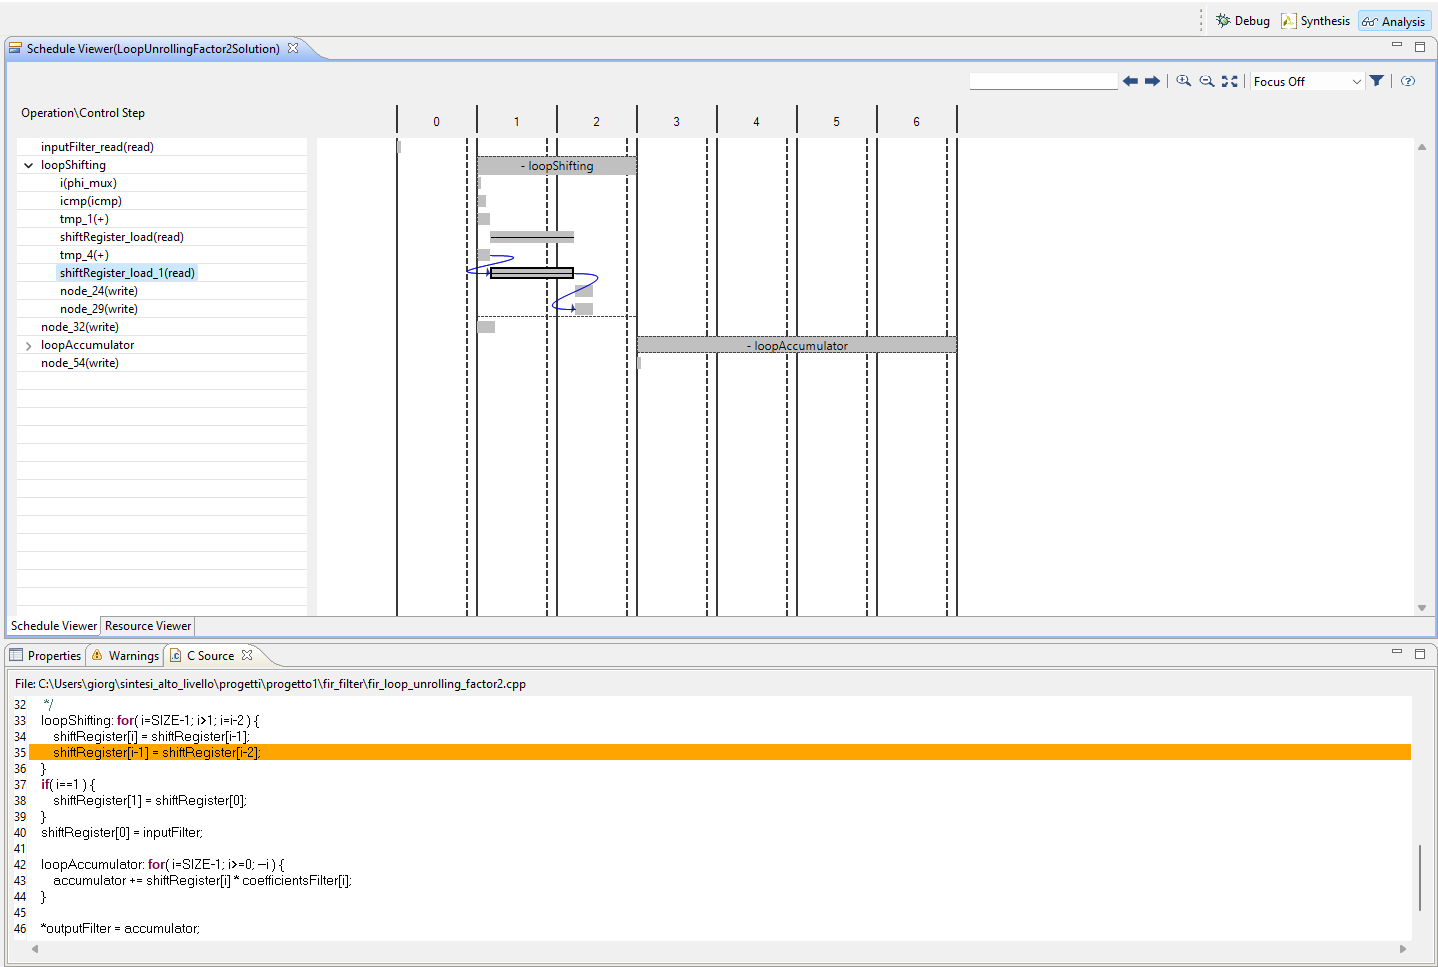
\includegraphics[width=0.9\textwidth]{solutions/loop_unrolling/factor2/loopunrollingmanual2.png}
    \caption{HLS Loop Unrolling Manual Factor=2 Analysis}
\end{figure}

\begin{figure}[H]
    \centering
    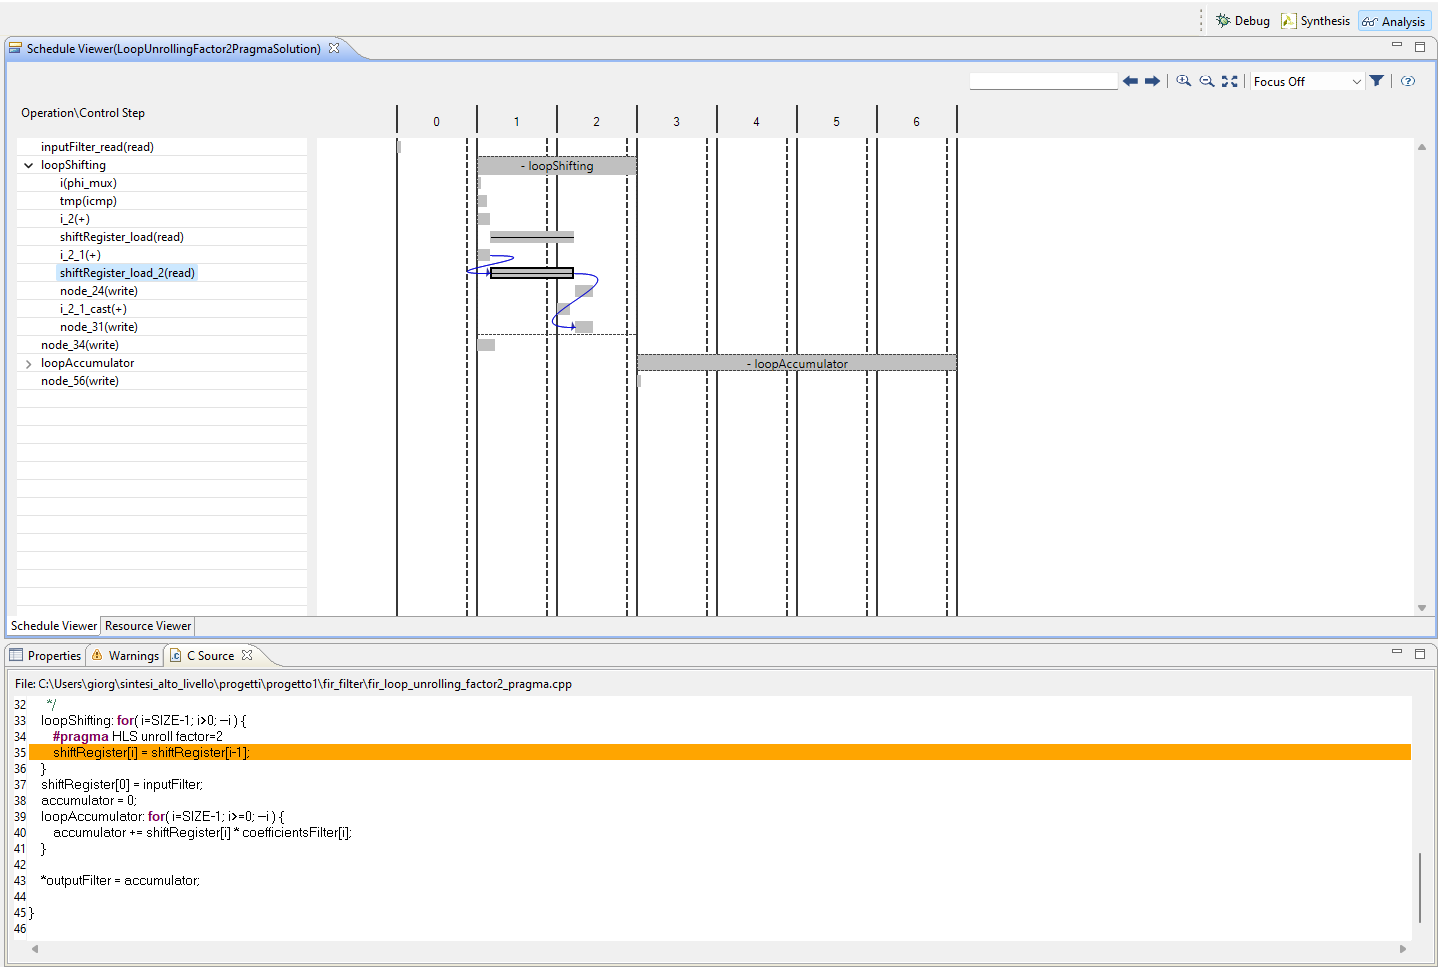
\includegraphics[width=0.9\textwidth]{solutions/loop_unrolling/factor2/loopunrollingautomatic2.png}
    \caption{HLS Loop Unrolling Automatic Factor=2 Analysis}
\end{figure}

Analizzando nel dettaglio il report si può notare come il numero di DSP e LUT sia pressocché il medesimo per tutte e tre le soluzioni hardware proposte. Per quanto riguarda, invece, il numero di BRAM utilizzate, le soluzioni basate su unrolling manuale e automatico presentano un'utilizzazione pari a 2, mentre quella basta su unrolling automatico e partitioning presenta un numero di BRAM utilizzato pari a 0. Questo è dovuto al fatto che il pragma di partizionamento, al fine di garantire accessi di read/write in memoria in parallelo, impone di non utilizzare le BRAM dual-port (che limiterebbero tali accessi). In particolare, impostando la tipologia di partizionamento \textit{complete}, la direttiva fa in modo che la soluzione hardware impieghi come memoria dei singoli registri, cosí che siano garantiti gli accessi in memoria in parallelo. Tanto è vero che si può notare un aumento considerevole dei FF in corrispondenza dell'architettura basata su unrolling automatico e partizionamento.

\begin{table}[H]
    \centering
    \begin{tabular}{|c|c|c|c|c|}
        \hline
        \textbf{Solution} & \textbf{BRAM\_18K} & \textbf{DSP48E} & \textbf{FF} & \textbf{LUT} \\
        \hline
        Manuale & 2 & 2 & 145 & 236 \\
        \hline
        Automatico & 2 & 2 & 141 & 251 \\
        \hline
        Automatico con Partitioning & 0 & 2 & 912 & 289 \\
        \hline
    \end{tabular}
    \caption{HLS Loop Unrolling Factor=2 Solution Utilization Estimates [\#]}
    \label{tab:hls-loop-unrolling-factor2-solution-utilization-report}
\end{table}

Qui di seguito vengono riportati i report relativi alla C/RTL Cosimulation, dove è possibile analizzare il numero di cicli di clock che servono per ottenere un risultato in uscita, e quello relativo a Export RTL.

\begin{table}[H]
    \centering
    \begin{tabular}{|c|c|c|c|c|c|c|c|c|}
        \hline
        \multicolumn{1}{|c|}{\textbf{Solution}} & \multicolumn{1}{|c|}{RTL} & \multicolumn{1}{|c|}{Status} & \multicolumn{3}{c|}{\textbf{Latency}} & \multicolumn{3}{c|}{\textbf{Interval}} \\
        & &  & min & avg & max & min & avg & max \\
        \hline
        Manuale & VHDL & Pass & 56 & 56 & 57 & 56 & 56 & 57 \\
        \hline
        Automatico & VHDL & Pass & 56 & 56 & 57 & 56 & 56 & 57 \\
        \hline
        Automatico con Partitioning & VHDL & Pass & 65 & 65 & 66 & 65 & 65 & 66 \\
        \hline
    \end{tabular}
    \caption{HLS Loop Unrolling Factor=2 Solution C/RTL Cosimulation Report }
    \label{tab:hls-loop-unrolling-factor2-solution-cosimulation-report}
\end{table}

\begin{table}[H]
    \centering
    \begin{tabular}{|c|c|c|c|c|c|c|c|c|}
        \hline
        \textbf{Solution} & \textbf{SLICE} & \textbf{LUT} & \textbf{FF} & \textbf{DSP} & \textbf{BRAM} & \textbf{CP} & \textbf{CP} & \textbf{CP} \\
        & & & & & & \textbf{required} & \textbf{achieved} & \textbf{achieved}\\
        & & & & & & & \textbf{post-} & \textbf{post-}\\
        & & & & & & & \textbf{synthesis} & \textbf{implementation}\\
        \hline
        Manuale & 31 & 97 & 72 & 2 & 2 & 10 & 5.745 & 5.692 \\
        \hline
        Automatico & 29 & 97 & 72 & 2 & 2 & 10 & 5.745 & 5.692 \\
        \hline
        Automatico  & 294 & 413 & 843 & 2 & 0 & 10 & 5.745 & 6.188 \\
        con Partitioning & & & & & & & & \\
        \hline
    \end{tabular}
    \caption{HLS Loop Unrolling Factor=2 Solution Export RTL Report}
    \label{tab:vivado-loop-unrolling-factor2-solution-export-rtl-report}
\end{table}


Pertanto, importando l'IP in Vivado e impostando un clock constraint pari a 10ns è possibile analizzare i seguenti report di risorse, timing, potenza dinamica ed energia per singola operazione.
\lstinputlisting[language=VHDL]{solutions/loop_unrolling/factor2/clk_constraint.xdc}

Analizzando il report di utilizzazione delle risorse generato da Vivado dopo aver effettuato il processo di implementazione, è possibile notare come il numero di risorse stimato dal tool HLS è leggermente mutato. Però, si può evidenziare come il cambiamento delle risorse tra le varie soluzioni hardware è il medesimo, cioè il numero di LUT e FF nel caso dell'implementazione con unrolling automatico e partitioning sia aumentato considerevolmente e il numero di BRAM si è ridotto a zero.

\begin{table}[H]
    \centering
    \begin{tabular}{|c|c|c|c|c|c|c|c|}
        \hline
        \textbf{Solution} & \textbf{LUT} & \textbf{LUTRAM} & \textbf{FF} & \textbf{BRAM} & \textbf{DSP} & \textbf{IO} & \textbf{BUFG} \\
        \hline
        Manuale & 98 & 0 & 72 & 1 & 2 & 71 & 1 \\
        \hline
        Automatico & 98 & 0 & 72 & 1 & 2 & 71 & 1 \\
        \hline
        Automatico & 413 & 0 & 843 & 0 & 2 & 71 & 1 \\
        con Partitioning & & & & & & & \\
        \hline
    \end{tabular}
    \caption{Vivado Loop Unrolling Factor=2 Solution Utilization Report [\#]}
    \label{tab:vivado-loop-unrolling-factor2-utilization-report}
\end{table}

Si è, inoltre, analizzato l'utilizzazione delle risorse effettuando un confronto con la soluzione hardware basata sulla scissione del loop dal momento che tali architetture basate su unrolling sono basate sulla prima citata. In particolare, si può notare come il numero di risorse utilizzate sia pressoché il medesimo tra la soluzione hardware basta su loop fission e quelle basate rispettivamente sull'unrolling manuale e automatico di fattore 2. Più nello specifico, considerando le implementazioni basate sul parallelismo manuale e automatico rispetto a quella basta sul loop fission, il numero di LUT è diminuito di circa il $40\%$, il numero di FF è diminuito di circa il $32\%$ e il numero di BRAM è aumentato di un'unità. Invece, effettuando un confronto tra quella basata su partitioning e quella basata sulla scissione del loop, il numero di LUT è aumentato di circa il $161\%$ e il numero di FF di circa il $695\%$.

\begin{figure}[H]
    \centering
    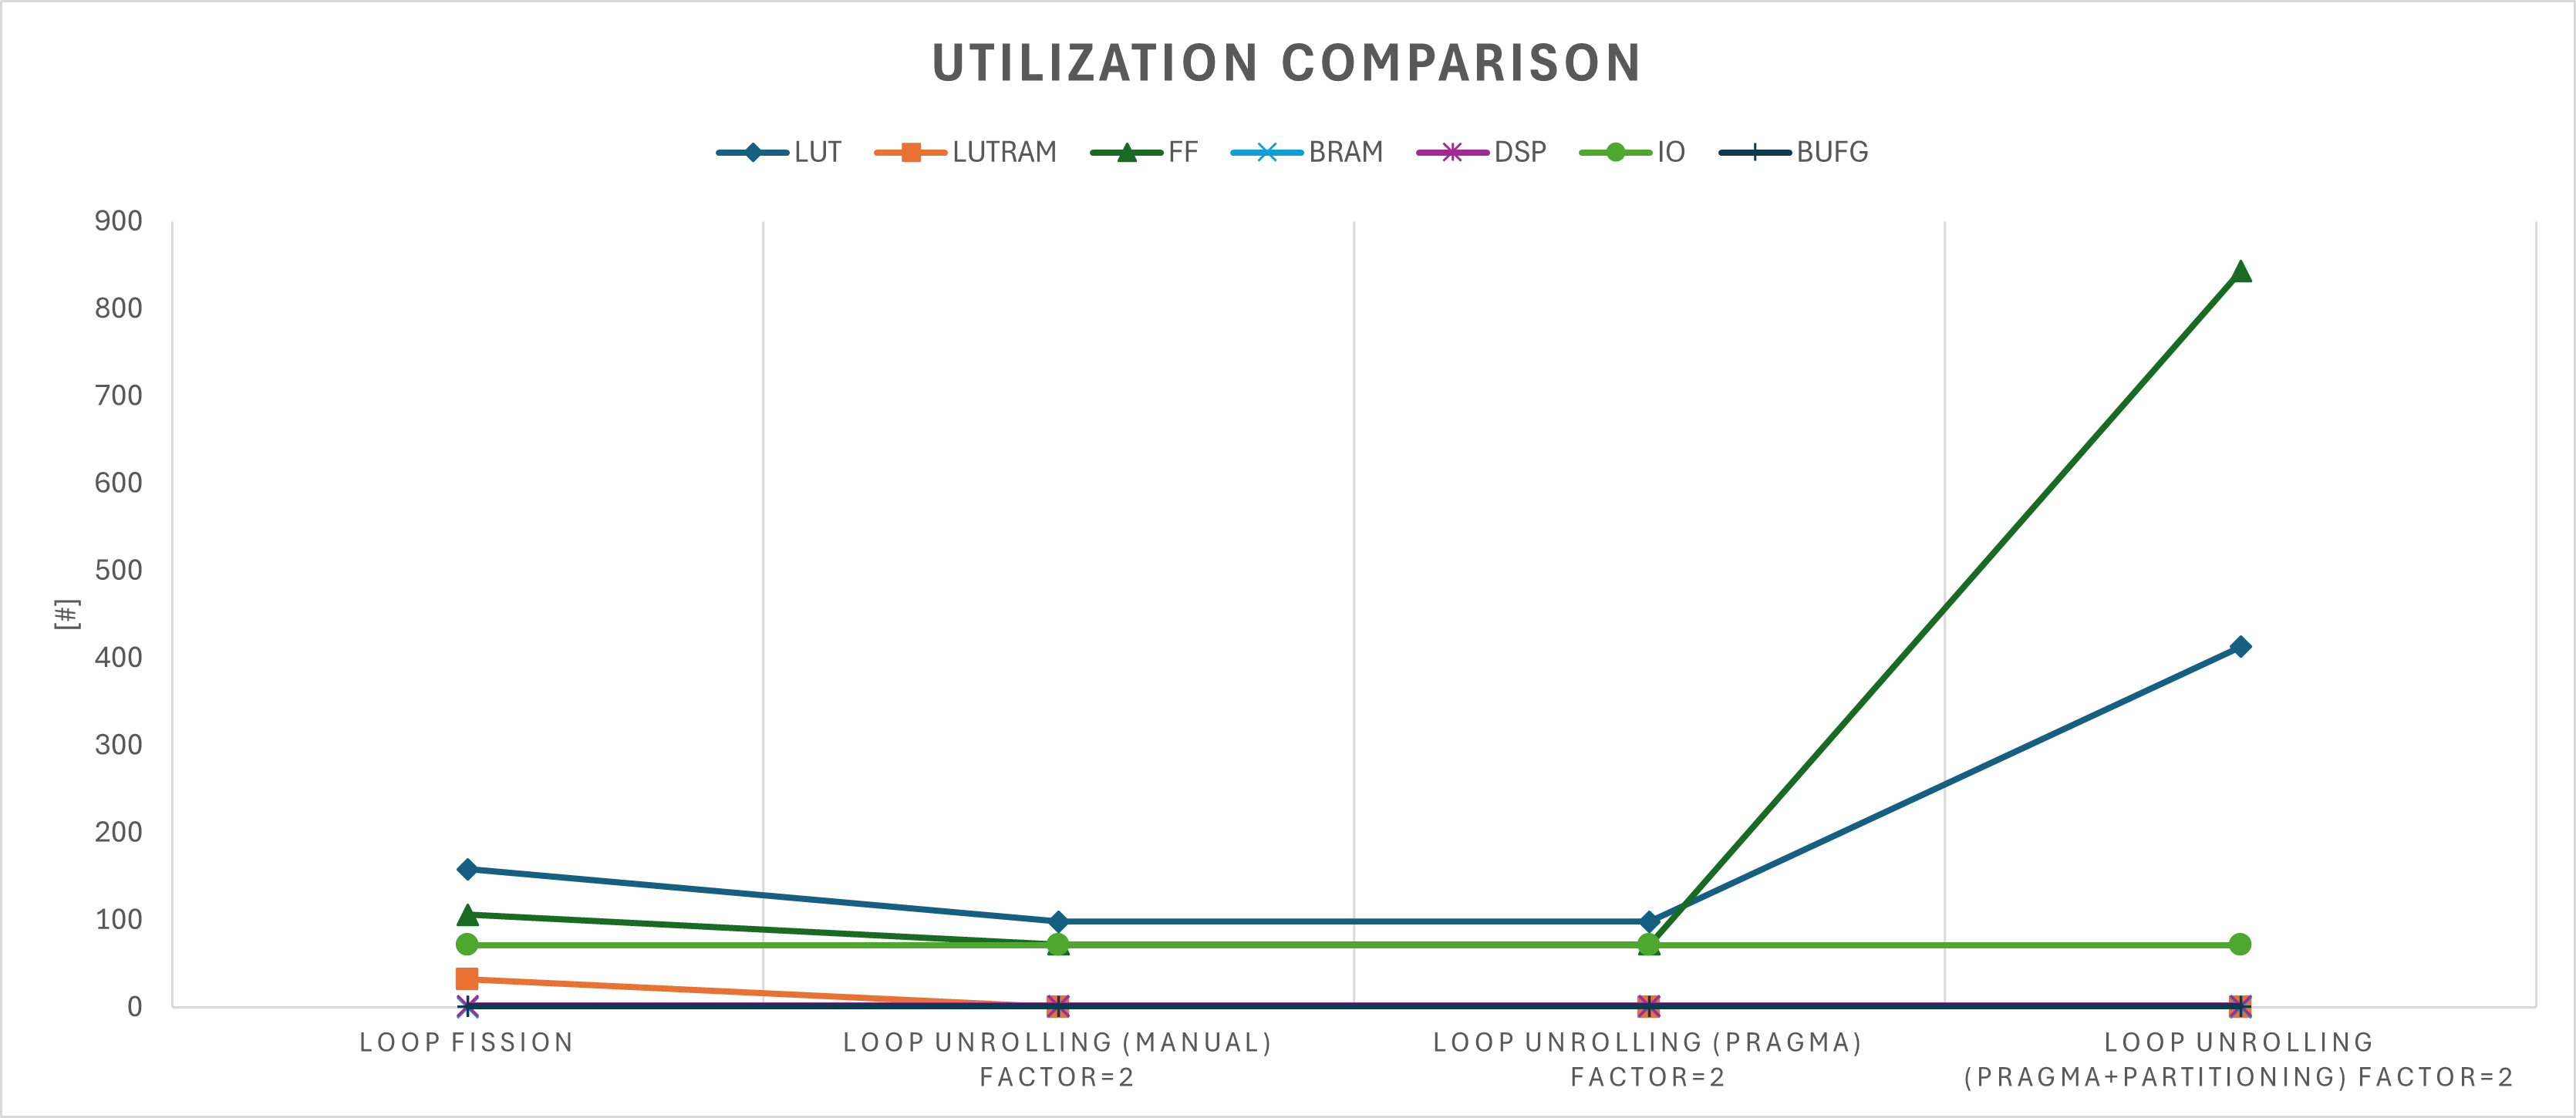
\includegraphics[width=0.9\textwidth]{solutions/loop_unrolling/factor2/loopunrollingfactor2utilization.png}
    \caption{Vivado Loop Unrolling Factor=2 Utilization Plot}
    \label{fig:vivado-loop-unrolling-factor2-utilization-plot}
\end{figure}

Infine, per quanto riguarda il timing, è possibile notare come il numero di cicli sia pressocché il medesimo tra la soluzione basata su unrolling manuale e quella basata su unrolling automatico. Invece, come precedentemente citato, la soluzione basata su partizionamento presenta un numero di cicli di clock, tali per garantire un risultato, maggiore.

\begin{table}[H]
    \centering
    \begin{tabular}{|c|c|c|c|c|}
        \hline
        \textbf{Solution} & \textbf{Cycles} [\#] & \textbf{Clock Constraint} [ns] & \textbf{WNS} [ns] & \textbf{Maximum Clock} \\
        & & & & \textbf{Frequency} [MHz] \\
        \hline
        Manuale & 57 & 10 & 4.33 & 176.366843 \\
        \hline
        Automatico & 57 & 10 & 4.33 & 176.366843 \\
        \hline
        Automatico & 66 & 10 & 3.469 & 153.1159087 \\
        con Partitioning & & & & \\
        \hline
    \end{tabular}
    \caption{Vivado Loop Unrolling Factor=2 Solution Timing Report}
    \label{tab:vivado-loop-unrolling-factor2-solution-timing-report}
\end{table}

Effettuando un confronto grafico e tenendo conto anche della soluzione basata sulla scissione del loop, è possibile evidenziare un numero di cicli di clock, tali per garantire un risultato, un WNS e una maximum clock frequency pressoché uguali tra l'implementazione basata su loop fission e quella basata su partizionamento. Questo accade dal momento che la soluzione hardware basata su unrolling automatico e partitioning fa diminuire il numero di cicli di clock tramite il parallelismo e lo fa aumentare allo stesso tempo a causa del partizionamento. 

\begin{figure}[H]
    \centering
    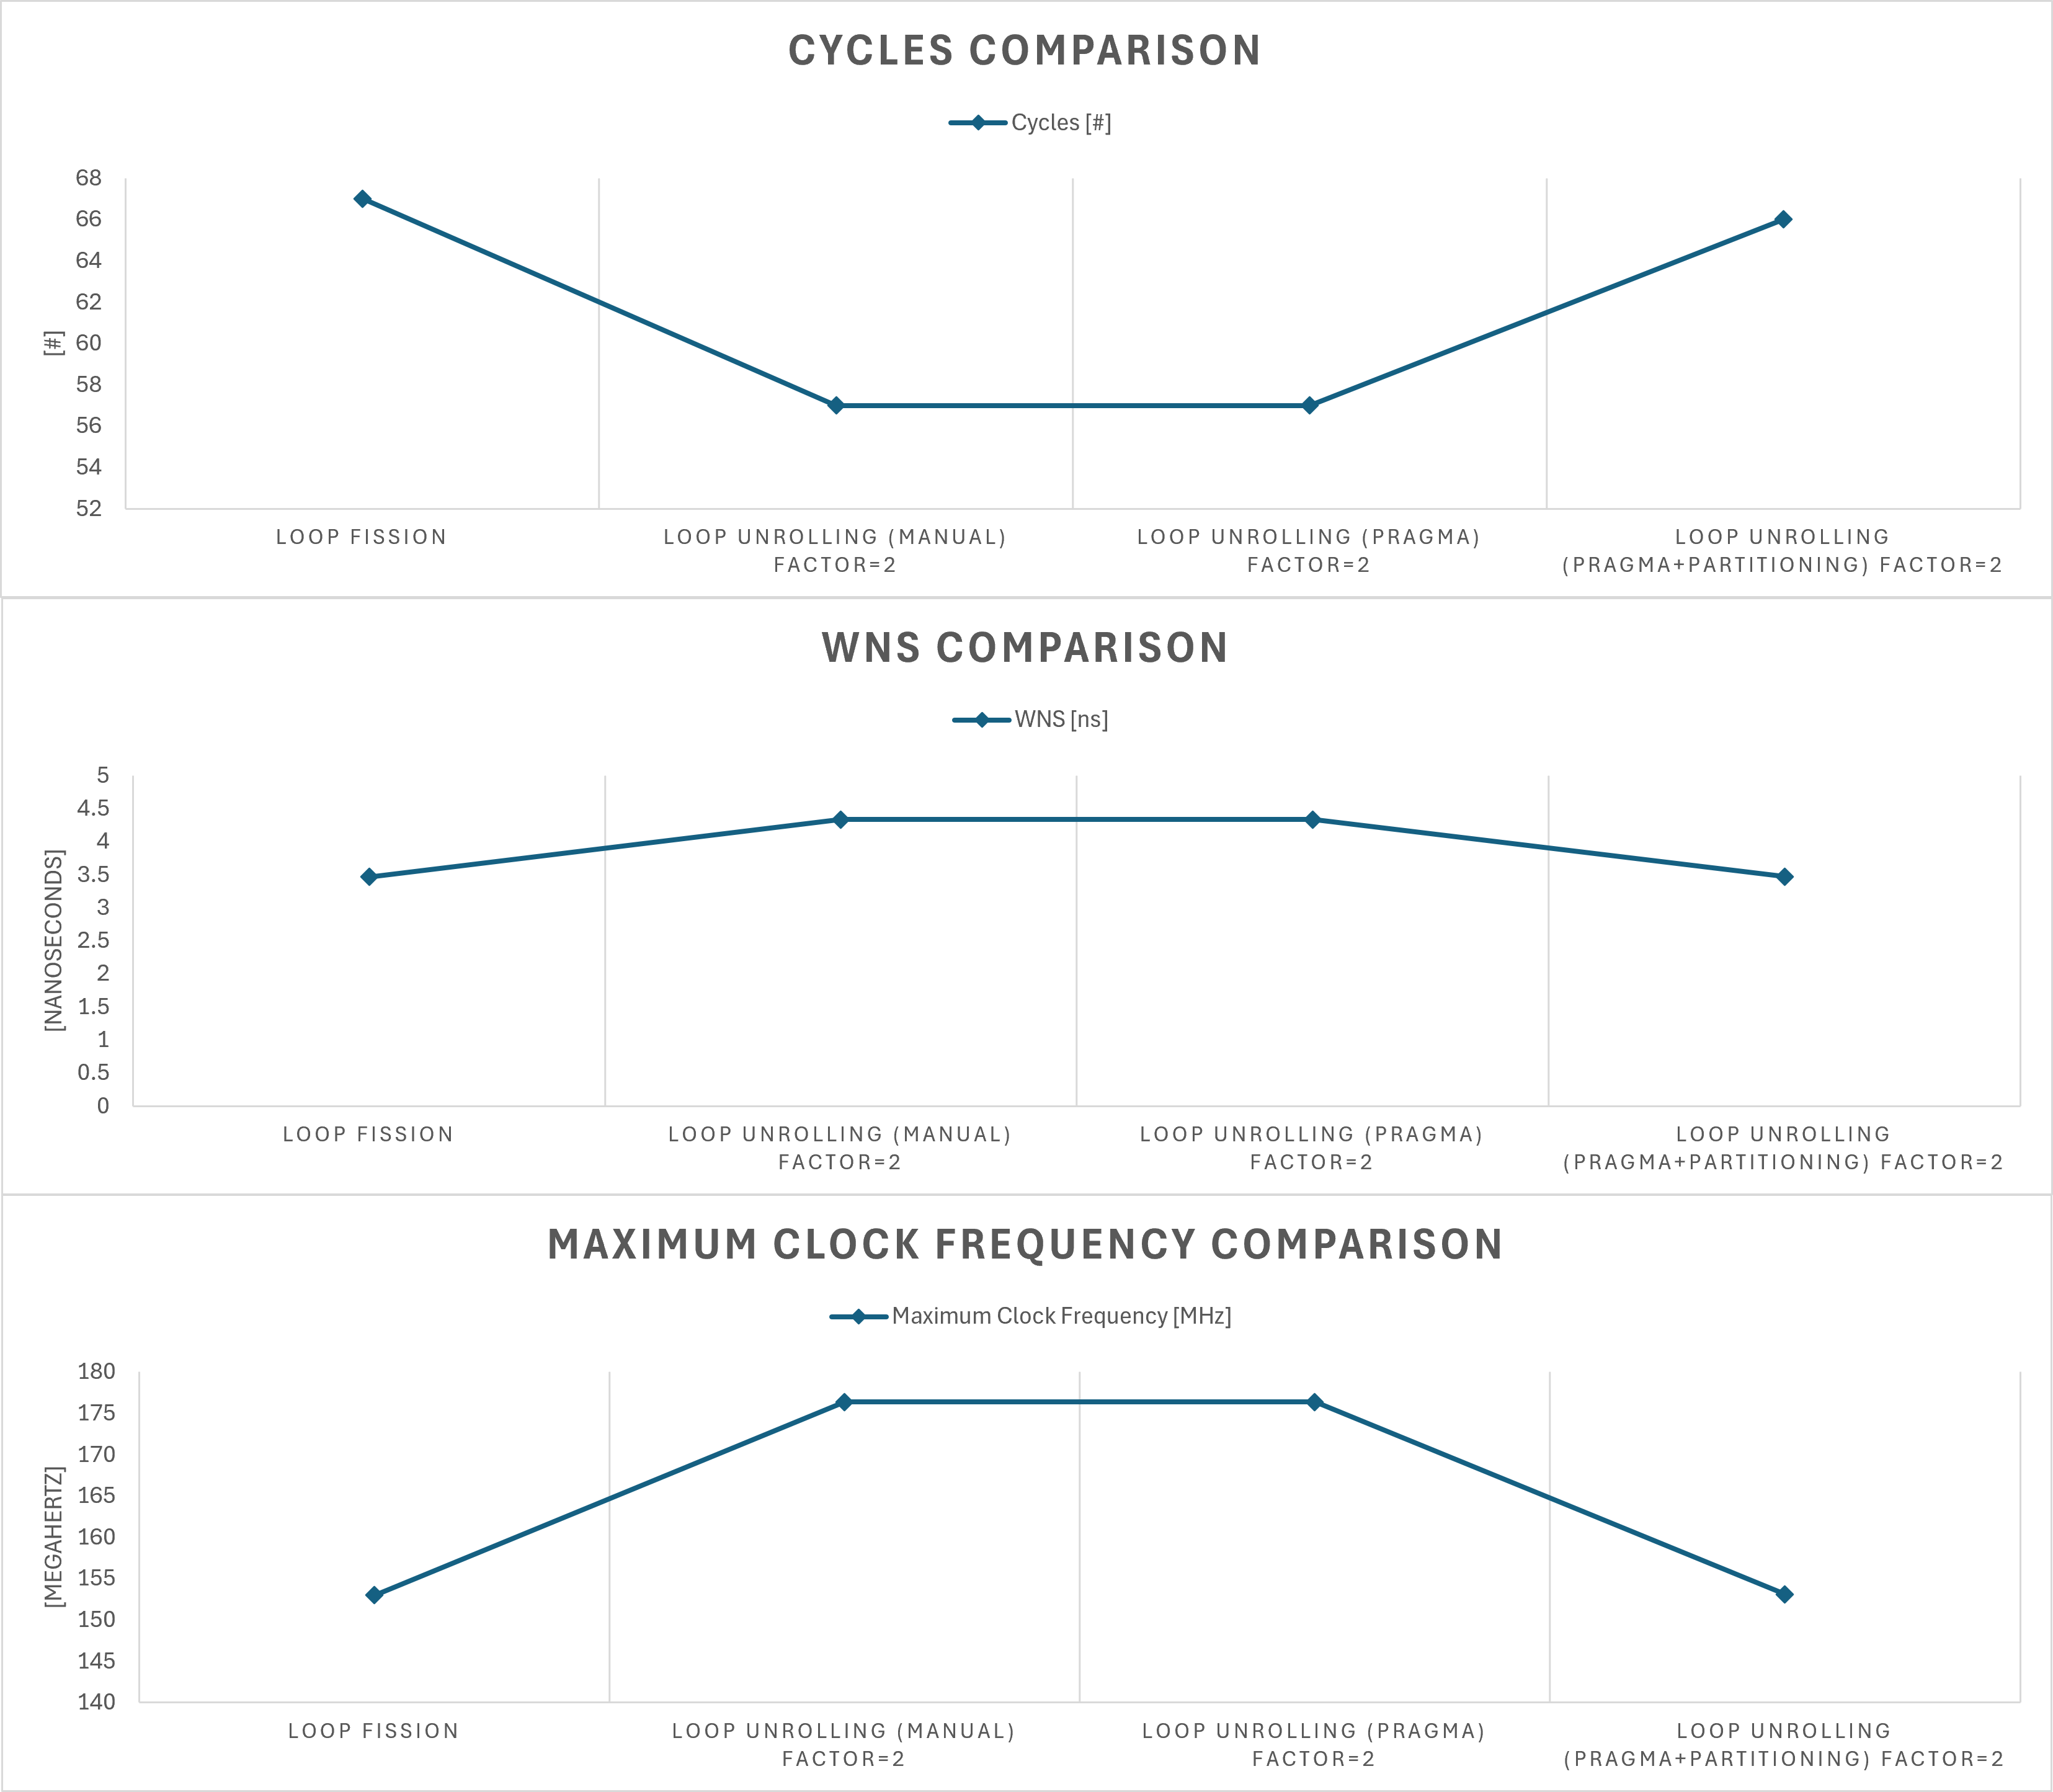
\includegraphics[width=0.8\textwidth]{solutions/loop_unrolling/factor2/loopunrollingfactor2timing.png}
    \caption{Vivado Loop Unrolling Factor=2 Timing Plot}
    \label{fig:vivado-loop-unrolling-factor2-solution-timing-plot}
\end{figure}

Per quanto riguarda, invece, la potenza dinamica associata alle tre soluzioni hardware proposte in questa sezione, è possibile notare come i contributi associati al Clock Enable e Clocks risultano essere notevolmente più grandi in corrispondenza dell'implementazione basata su partizionamento. Questo potrebbe essere causato dal notevole aumento dell'utilizzazione dei FF per questa solution. 

\begin{table}[H]
    \centering
    \begin{tabular}{|c|c|c|c|c|c|c|c|}
        \hline
        \textbf{Solution} & \textbf{BRAM} & \textbf{Clock} & \textbf{Clocks} & \textbf{DSP} & \textbf{Logic} & \textbf{Set/}& \textbf{Data} \\
        & & \textbf{Enable} & & & & \textbf{Reset} & \\
        \hline
        Manuale & 1.250551548 & 0.096387172 & 0.900532817 & 0.268251897 & 0.260709843 & 0.003146866 & 0.423992984 \\
        \hline
        Automatico & 1.240851358 & 0.082524632 & 0.960682868 & 0.272355421 & 0.266662013 & 0.00428147 & 0.425589533 \\
        \hline
        Automatico & & & & & & & \\
        con & 0 & 0.325270201 & 2.352835611 & 0.263715046 & 0.575191109 & 0.007010513 & 0.750690058 \\
        Partitioning & & & & & & & \\
        \hline
    \end{tabular}
    \caption{Vivado Loop Unrolling Factor=2 Solution Dynamic Power Report [mW]}
    \label{tab:vivado-loop-unrolling-factor2-solution-dynamic-power-reproot}
\end{table}

Infatti, è possibile riscontrare un aumento della potenza dinamica totale e dell'energia per singola operazione in corrispondenza dell'architettura basata su unrolling e partitioning. Invece, per quanto riguarda le altre due solution (unrolling manuale e automatico), entrambi i parametri appena citati risultano essere i medesimi. 

\begin{table}[H]
    \centering
    \begin{minipage}[t]{0.45\linewidth}
        \centering
        \begin{tabular}{|c|c|}
            \hline
            \textbf{Solution} & \textbf{Dynamic Total} \\
            \hline
            Manuale & 3.203573127 \\
            \hline
            Automatico & 3.252947294 \\
            \hline
            Automatico & 4.274712538 \\
            con Partitioning & \\
            \hline
        \end{tabular}
        \caption{Vivado Loop Unrolling Factor=2 Solution Dynamic Power Report [mW]}
        \label{tab:vivado-loop-unrolling-factor2-solution-dynamic-power-reproot}
    \end{minipage}
    \hfill
    \centering
    \begin{minipage}[t]{0.45\linewidth}
        \centering
        \begin{tabular}{|c|c|}
            \hline
            \textbf{Solution} & \textbf{Energy Single Operation} \\
            \hline
            Manuale & 32.03573127 \\
            \hline
            Automatico & 32.52947294 \\
            \hline
            Automatico & 42.74712538 \\
            con Partitioning & \\
            \hline
        \end{tabular}
        \caption{Vivado Loop Unrolling Factor=2 Solution Energy Single Operation Report [pJ]}
        \label{tab:vivado-loop-unrolling-factor2-solution-solution-energy-single-operation-reproot}
    \end{minipage}
\end{table}

Analizzando graficamente queste tre soluzioni e in aggiunta anche l'implementazione basata sulla scissione del loop, è possibile notare come quella basasta su loop fission presenta un medesimo valore di potenza dinamica totale ed energia per singola operazione rispetto alle due soluzioni di unrolling manuale e automatico.

\begin{figure}[H]
    \centering
    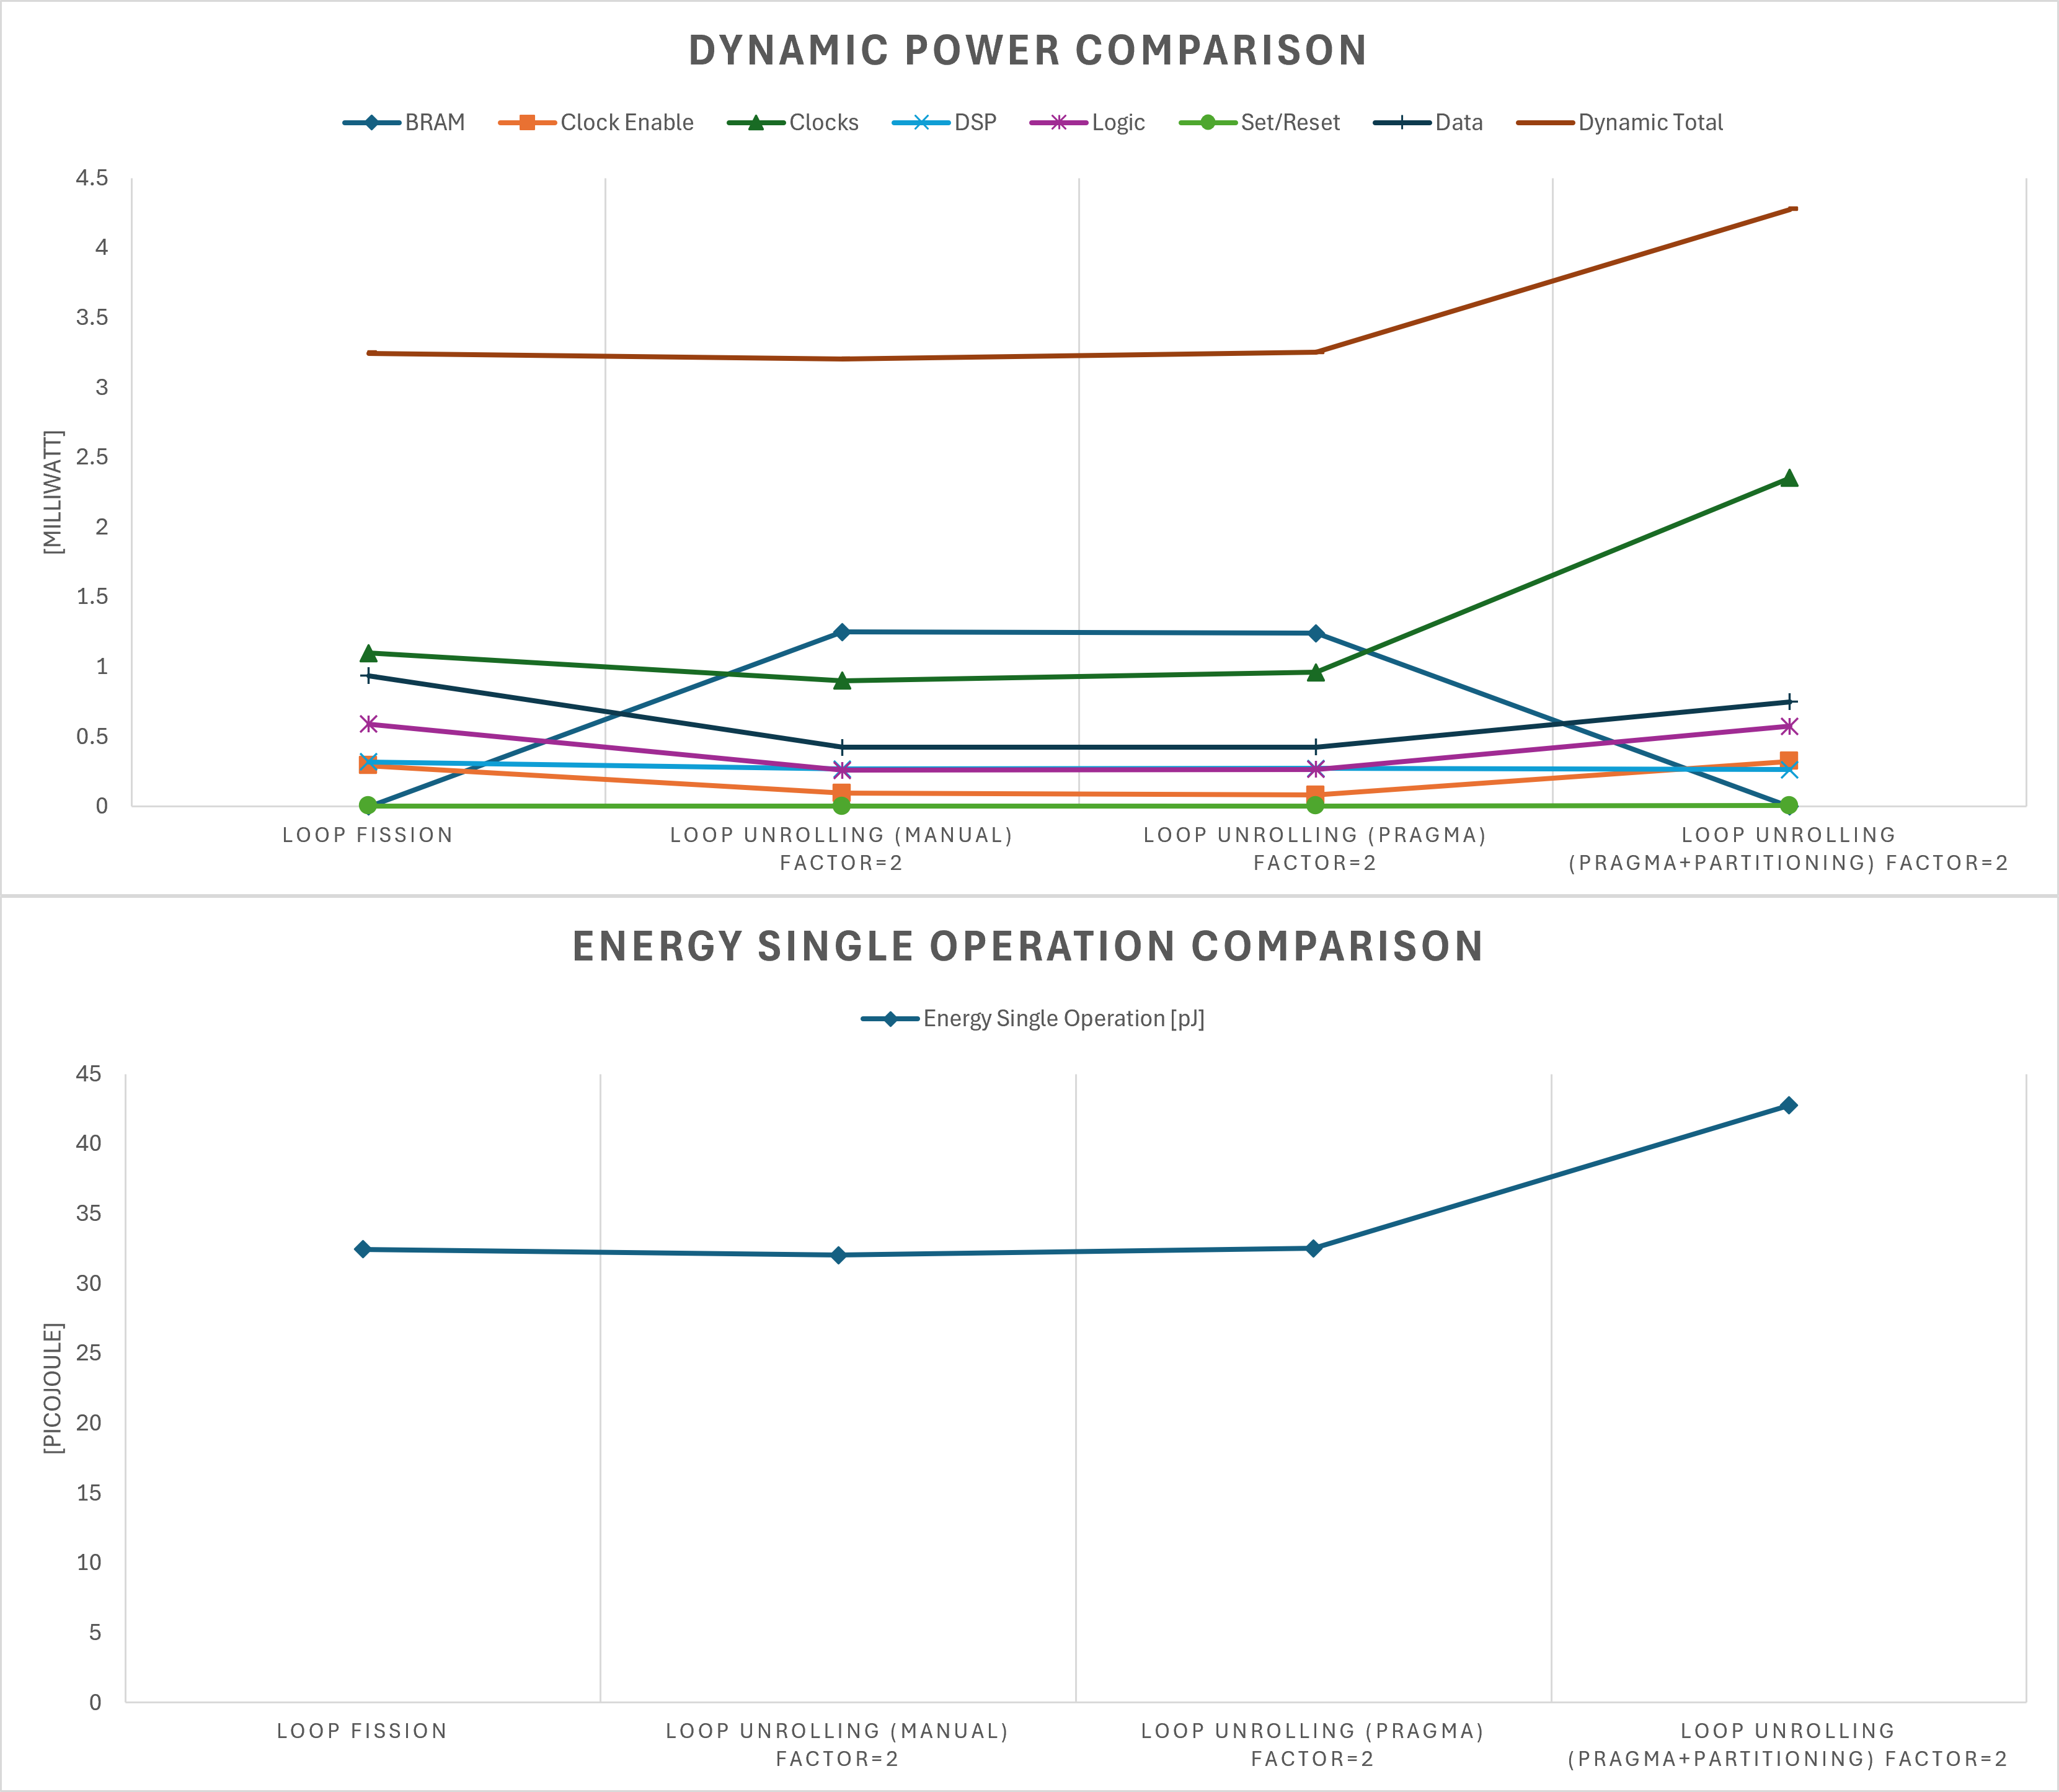
\includegraphics[width=\textwidth]{solutions/loop_unrolling/factor2/loopunrollingfactor2power.png}
    \caption{Vivado Loop Unrolling Factor=2 Dynamic Power Plot}
    \label{fig:vivado-loop-unrolling-factor2-solution-power-plot}
\end{figure}


\newpage

\subsubsection{Loop Unrolling Factor=4}
\lstinputlisting[language=C++]{solutions/loop_unrolling/factor4/fir_loop_unrolling_manual_factor4.cpp}
\lstinputlisting[language=C++]{solutions/loop_unrolling/factor4/fir_loop_unrolling_automatic_factor4.cpp}
\lstinputlisting[language=C++]{solutions/loop_unrolling/factor4/fir_loop_unrolling_automatic_partiotioning_factor4.cpp}

\begin{table}[H]
    \centering
    \begin{tabular}{|c|c|c|c|c|}
        \hline
        \textbf{Solution} & \textbf{Clock} & \textbf{Target} & \textbf{Estimated} & \textbf{Uncertainty} \\
        \hline
        Manuale & ap\_clk & 10.00 & 8.510 & 1.25 \\
        \hline
        Automatico & ap\_clk & 10.00 & 8.510 & 1.25 \\
        \hline
        Automatico con Partitioning & ap\_clk & 10.00 & 8.510 & 1.25 \\
        \hline
    \end{tabular}
    \caption{HLS Loop Unrolling Factor=4 Solution Timing Summary (ns)}
    \label{tab:hls-loop-unrolling-factor4-solution-timing-summary}
\end{table}

\begin{table}[H]
    \centering
    \begin{tabular}{|c|c|c|c|c|}
        \hline
        \multicolumn{1}{|c|}{\textbf{Solution}} & \multicolumn{2}{|c|}{\textbf{Latency}} & \multicolumn{2}{|c|}{\textbf{Interval}} \\
        & min & max & min & max \\
        \hline
        Manuale & 58 & 58 & 58 & 58 \\
        \hline
        Automatico & 62 & 66 & 62 & 66 \\
        \hline
        Automatico con Partitioning & 62 & 64 & 62 & 64 \\
        \hline
    \end{tabular}
    \caption{HLS Loop Unrolling Factor=4 Solution Latency Summary (clock cycles)}
    \label{tab:hls-loop-unrolling-factor4-solution-latency-summary}
\end{table}

\begin{table}[H]
    \centering
    \begin{tabular}{|c|c|c|c|c|c|c|c|c|c|}
        \hline
        \multicolumn{1}{|c|}{\textbf{Solution}} & \multicolumn{1}{|c|}{Loop Name} & \multicolumn{2}{|c|}{\textbf{Latency}} & \multicolumn{2}{c|}{\textbf{Iteration Latency}} & \multicolumn{2}{c|}{\textbf{Initiation Interval}} & \multicolumn{1}{c|}{\textbf{Trip}}  \\
        &  & min & max & min & max & achieved & target & \textbf{Count} \\
        \hline
        Manuale & - loopShifting & 12 & 12 & 4 & 4 & - & - & 3 \\
        & - loopAccumulator & 44 & 44 & 4 & 4 & - & - & 11 \\
        \hline
        Automatico & - loopShifting & 15 & 18 & 5 & 5 & - & - & 3 \\
        & - loopAccumulator & 44 & 44 & 4 & 4 & - & - & 11 \\
        \hline
        Automatico  & - loopShifting & 15 & 17 & 5 & 5 & - & - & 3 \\
        con Partitioning & - loopAccumulator & 44 & 44 & 4 & 4 & - & - & 11 \\
        \hline
    \end{tabular}
    \caption{HLS Loop Unrolling Factor=4 Solution Latency Loops Summary }
    \label{tab:hls-loop-unrolling-factor4-solution-loop-summary}
\end{table}

In questo caso si può notare come il trip count sia, ovviamente, il medesimo per tutte e tre le soluzioni. Ciò che cambia effettivamente, come nel caso del fattore pari a 2, è la latency associata ai loop. In particolare, analizzando più nel dettaglio, tramite l'interfaccia Analysis, si può evidenziare come il loopShifting, in cui viene implementato un parallelismo pari a 4, viene gestito in maniera differente. Infatti, nel caso del loop unrolling manuale, vengono effettuate in parallelo due read alla volta e poi successivamente vengono eseguite in parallelo due write alla volta. Invece, nel caso della soluzione hardware basata su unrolling automatico, vengono effettuate una read e una write in parallelo per ogni ciclo di latenza. Nello specifico, considerando quattro shifting per ogni iterazione, viene effettuata la read al primo ciclo di latenza e, successivamente, viene eseguita la write corrispondente in parallelo alla read relativo al secondo shifting e così via. Di conseguenza, si avranno cinque colpi di latenza per ogni iterazione come riportato dal valore di iteration latency del report di sintesi.

\begin{figure}[H]
    \centering
    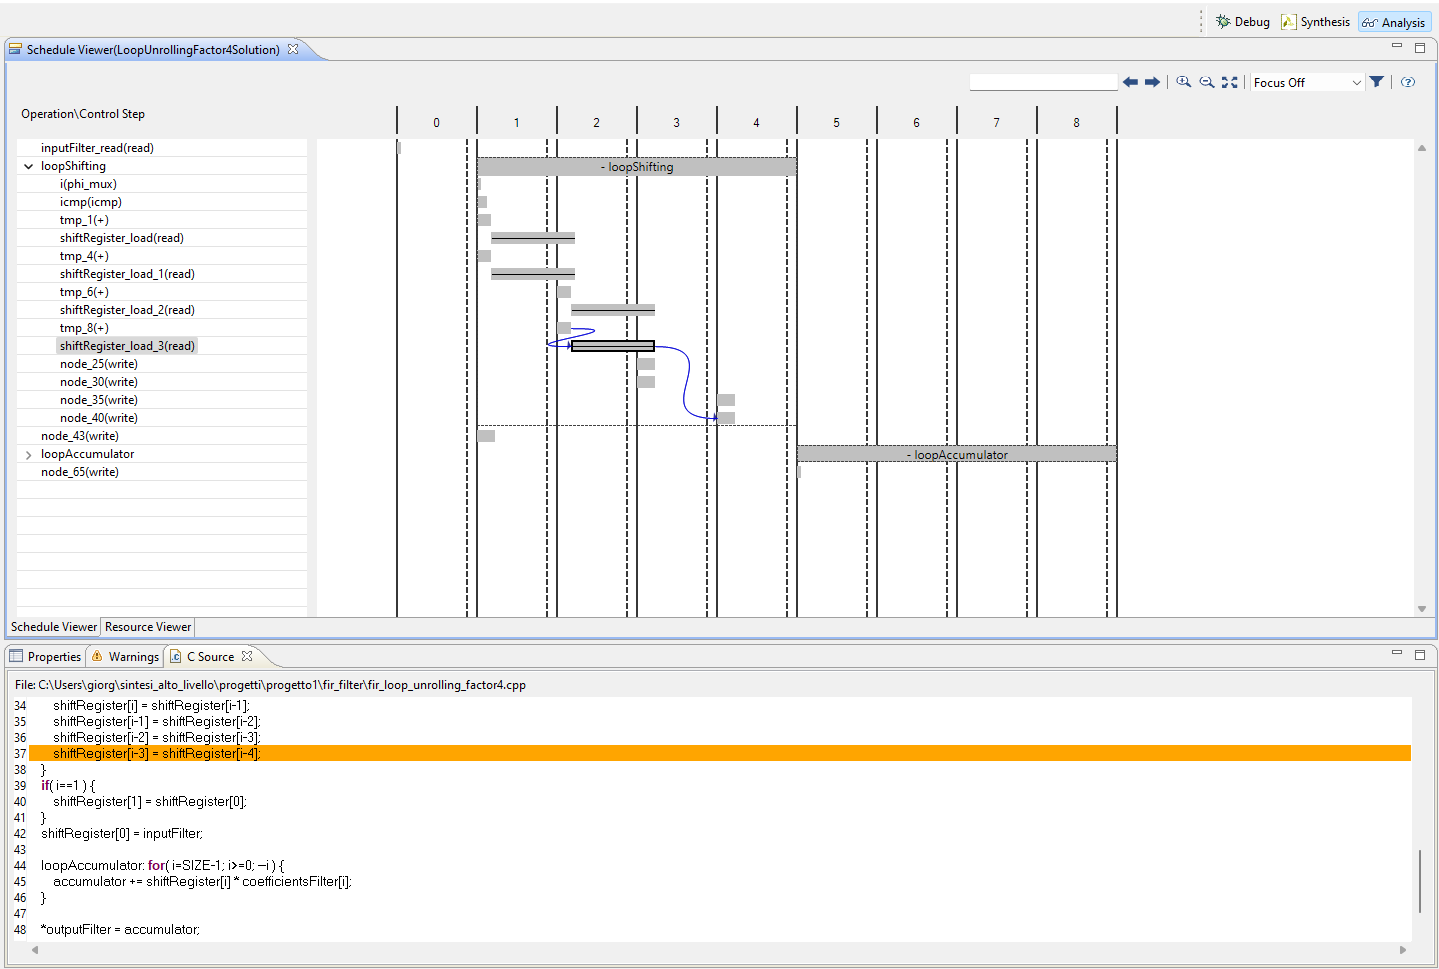
\includegraphics[width=0.9\textwidth]{solutions/loop_unrolling/factor4/loopunrollingmanual4.png}
    \caption{HLS Loop Unrolling Manual Factor=4 Analysis}
\end{figure}

\begin{figure}[H]
    \centering
    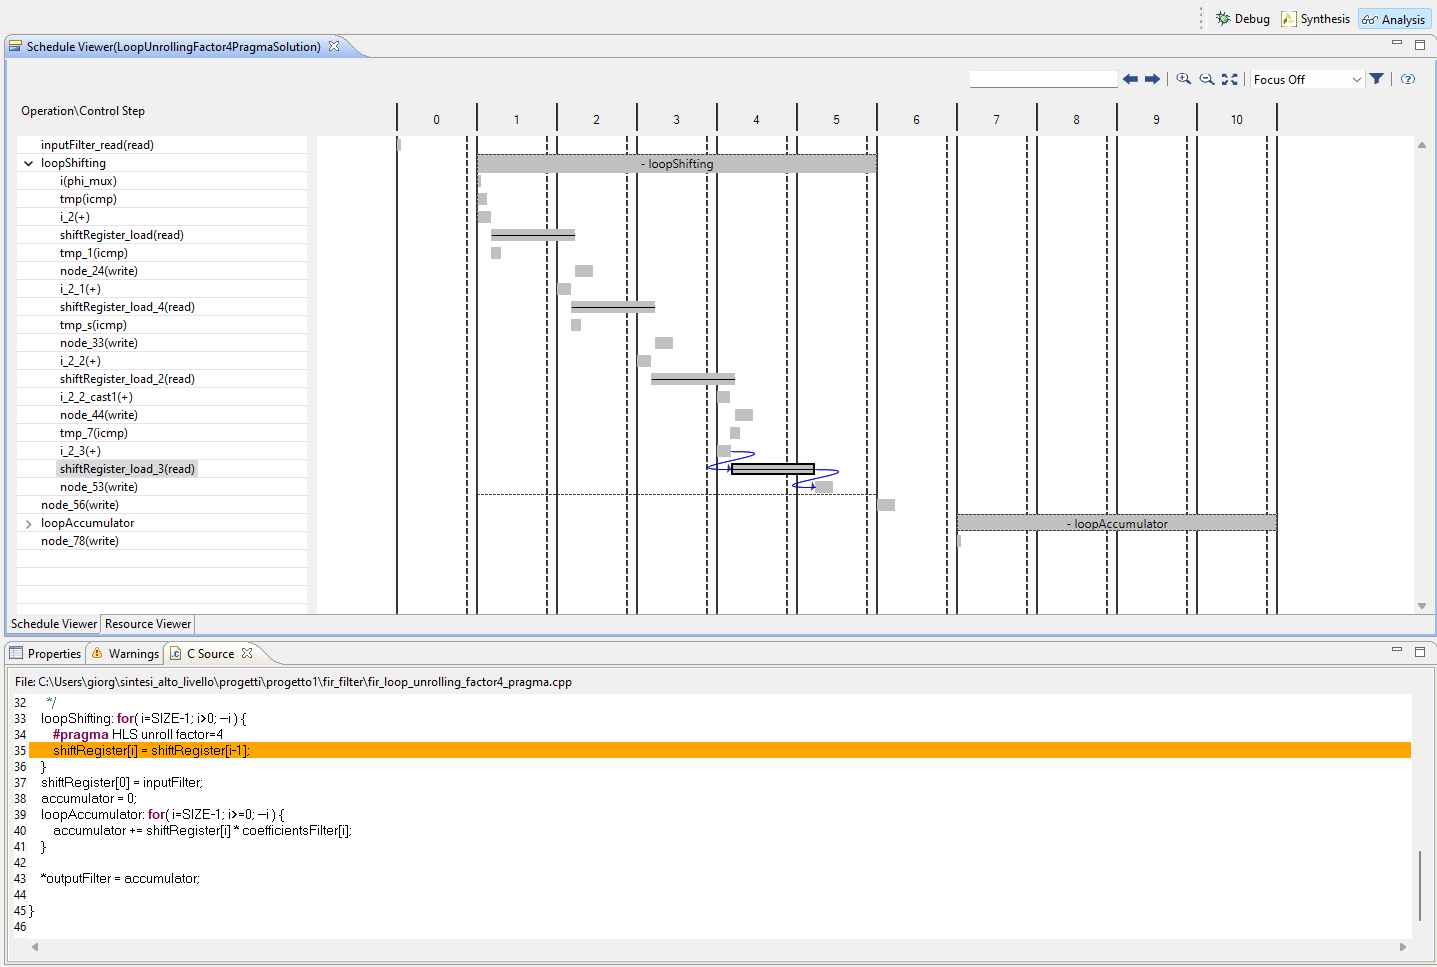
\includegraphics[width=0.9\textwidth]{solutions/loop_unrolling/factor4/loopunrollingautomatic4.png}
    \caption{HLS Loop Unrolling Automatic Factor=4 Analysis}
\end{figure}

Analogamente a quanto è stato analizzato e descritto nel caso di parallelismo di fattore pari a 2, anche in questo caso si può notare come l'utilizzazione delle risorse sia quasi la medesima tra il loop unrolling manuale e automatico. Invece, per quanto riguarda il loop unrolling automatico con partitioning, si ha un notevole aumento dell'utilizzazione sia di FF sia di LUT.

\begin{table}[H]
    \centering
    \begin{tabular}{|c|c|c|c|c|}
        \hline
        \textbf{Solution} & \textbf{BRAM\_18K} & \textbf{DSP48E} & \textbf{FF} & \textbf{LUT} \\
        \hline
        Manuale & 2 & 2 & 221 & 318 \\
        \hline
        Automatico & 2 & 2 & 194 & 367 \\
        \hline
        Automatico con Partitioning & 0 & 2 & 928 & 748 \\
        \hline
    \end{tabular}
    \caption{HLS Loop Unrolling Factor=4 Solution Utilization Estimates [\#]}
    \label{tab:vivado-loop-unrolling-factor4-solution-utilization-report}
\end{table}

Qui di seguito vengono riportati i report relativi alla C/RTL Cosimulation, dove è possibile analizzare il numero di cicli di clock che servono per ottenere un risultato in uscita, e quello relativo a Export RTL.

\begin{table}[H]
    \centering
    \begin{tabular}{|c|c|c|c|c|c|c|c|c|}
        \hline
        \multicolumn{1}{|c|}{\textbf{Solution}} & \multicolumn{1}{|c|}{RTL} & \multicolumn{1}{|c|}{Status} & \multicolumn{3}{c|}{\textbf{Latency}} & \multicolumn{3}{c|}{\textbf{Interval}} \\
        & &  & min & avg & max & min & avg & max \\
        \hline
        Manuale & VHDL & Pass & 58 & 58 & 59 & 58 & 58 & 59 \\
        \hline
        Automatico & VHDL & Pass & 60 & 60 & 61 & 60 & 60 & 61 \\
        \hline
        Automatico con Partitioning & VHDL & Pass & 58 & 58 & 59 & 58 & 58 & 59 \\
        \hline
    \end{tabular}
    \caption{HLS Loop Unrolling Factor=4 Solution C/RTL Cosimulation Report }
    \label{tab:hls-loop-unrolling-factor4-solution-cosimulation-report}
\end{table}

\begin{table}[H]
    \centering
    \begin{tabular}{|c|c|c|c|c|c|c|c|c|}
        \hline
        \textbf{Solution} & \textbf{SLICE} & \textbf{LUT} & \textbf{FF} & \textbf{DSP} & \textbf{BRAM} & \textbf{CP} & \textbf{CP} & \textbf{CP} \\
        & & & & & & \textbf{required} & \textbf{achieved} & \textbf{achieved}\\
        & & & & & & & \textbf{post-} & \textbf{post-}\\
        & & & & & & & \textbf{synthesis} & \textbf{implementation}\\
        \hline
        Manuale & 46 & 160 & 147 & 2 & 2 & 10 & 5.745 & 5.692 \\
        \hline
        Automatico & 40 & 145 & 93 & 2 & 2 & 10 & 5.745 & 5.692 \\
        \hline
        Automatico  & 412 & 1145 & 864 & 2 & 0 & 10 & 5.745 & 7.109 \\
        con Partitioning & & & & & & & & \\
        \hline
    \end{tabular}
    \caption{HLS Loop Unrolling Factor=4 Solution Export RTL Report}
    \label{tab:vivado-loop-unrolling-factor4-solution-export-rtl-report}
\end{table}

Pertanto, importando l'IP in Vivado e impostando un clock constraint pari a 10ns è possibile analizzare i seguenti report di risorse, timing, potenza dinamica ed energia per singola operazione.
\lstinputlisting[language=VHDL]{solutions/loop_unrolling/factor2/clk_constraint.xdc}

Analogamente all'unrolling di fattore pari a 2, anche in questo caso in corrispondenza della soluzione hardware basata su unrolling e partizionamento si ha un notevole aumento di utilizzazione delle risorse. Inoltre, si può notare come il numero di FF utilizzati per la solution di unrolling automatico risulta essere circa il $37\%$ in meno rispetto a quella basata su unrolling manuale. Evidentemente il tool, tramite la direttiva proprietaria, è riuscito ad effettuare delle ottimizzazione tali da garantire una diminuzione dei Flip Flop.

\begin{table}[H]
    \centering
    \begin{tabular}{|c|c|c|c|c|c|c|c|}
        \hline
        \textbf{Solution} & \textbf{LUT} & \textbf{LUTRAM} & \textbf{FF} & \textbf{BRAM} & \textbf{DSP} & \textbf{IO} & \textbf{BUFG} \\
        \hline
        Manuale & 159 & 0 & 147 & 1 & 2 & 71 & 1 \\
        \hline
        Automatico & 145 & 0 & 93 & 1 & 2 & 71 & 1 \\
        \hline
        Automatico & 1145 & 0 & 864 & 0 & 2 & 71 & 1 \\
        con Partitioning & & & & & & & \\
        \hline
    \end{tabular}
    \caption{Vivado Loop Unrolling Factor=4 Solution Utilization Report [\#]}
    \label{tab:vivado-loop-unrolling-factor4-utilization-report}
\end{table}

Effettuando un confronto grafico e tenendo conto dei dati precedentemente ottenuti per la soluzione basata su scissione del loop, si può notare come l'utilizzazione delle risorse sia pressocché la medesima tra loop fission e loop unrolling automatico.

\begin{figure}[H]
    \centering
    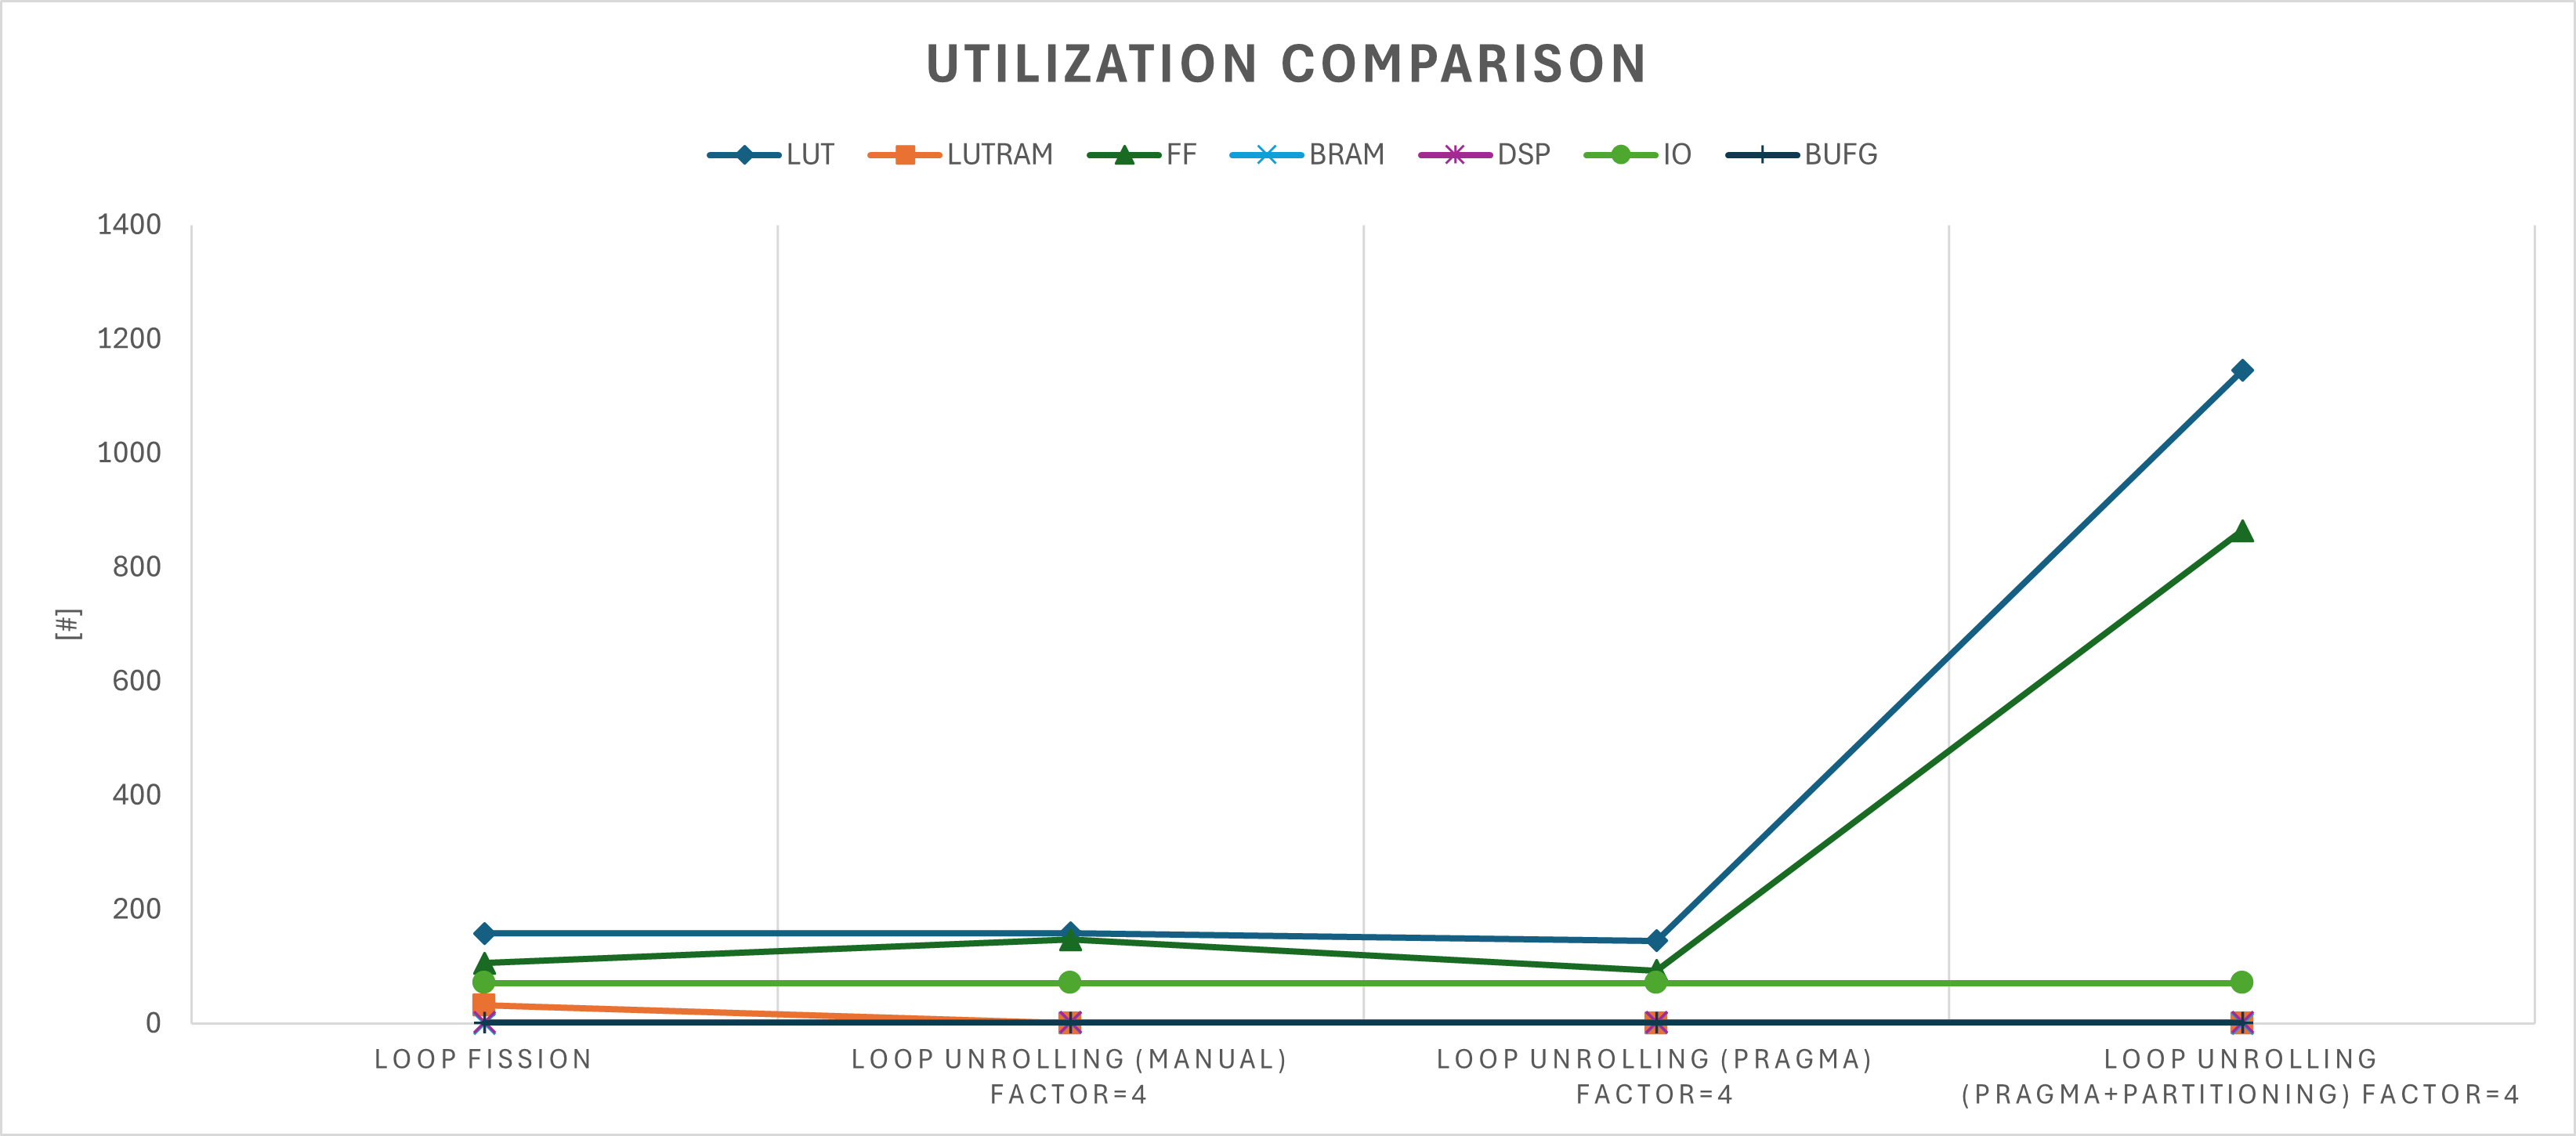
\includegraphics[width=0.9\textwidth]{solutions/loop_unrolling/factor4/loopunrollingfactor4utilization.png}
    \caption{Vivado Loop Unrolling Factor=4 Utilization Plot}
    \label{fig:vivado-loop-unrolling-factor4-utilization-plot}
\end{figure}

Per quanto riguarda il report di timing, è possibile notare, analogamente a quanto successo per l'unrolling di fattore pari a 2, una diminuzione della maximum clock frequency in corrispondenza della soluzione basata su loop unrolling automatico con partizionamento.

\begin{table}[H]
    \centering
    \begin{tabular}{|c|c|c|c|c|}
        \hline
        \textbf{Solution} & \textbf{Cycles} [\#] & \textbf{Clock Constraint} [ns] & \textbf{WNS} [ns] & \textbf{Maximum Clock} \\
        & & & & \textbf{Frequency} [MHz] \\
        \hline
        Manuale & 59 & 10 & 4.257 & 174.1250218 \\
        \hline
        Automatico & 61 & 10 & 4.33 & 176.366843 \\
        \hline
        Automatico & 59 & 10 & 3.097 & 144.8645516 \\
        con Partitioning & & & & \\
        \hline
    \end{tabular}
    \caption{Vivado Loop Unrolling Factor=4 Solution Timing Report}
    \label{tab:vivado-loop-unrolling-factor4-solution-timing-report}
\end{table}

Per quanto riguarda, invece, il numero di cicli di clock per garantire un risultato in uscita, in questo caso, per le tre soluzioni basate su unrolling di fattore pari a 4, si è ottenuto un valore minore rispetto alla soluzione basata su scissione del loop. 

\begin{figure}[H]
    \centering
    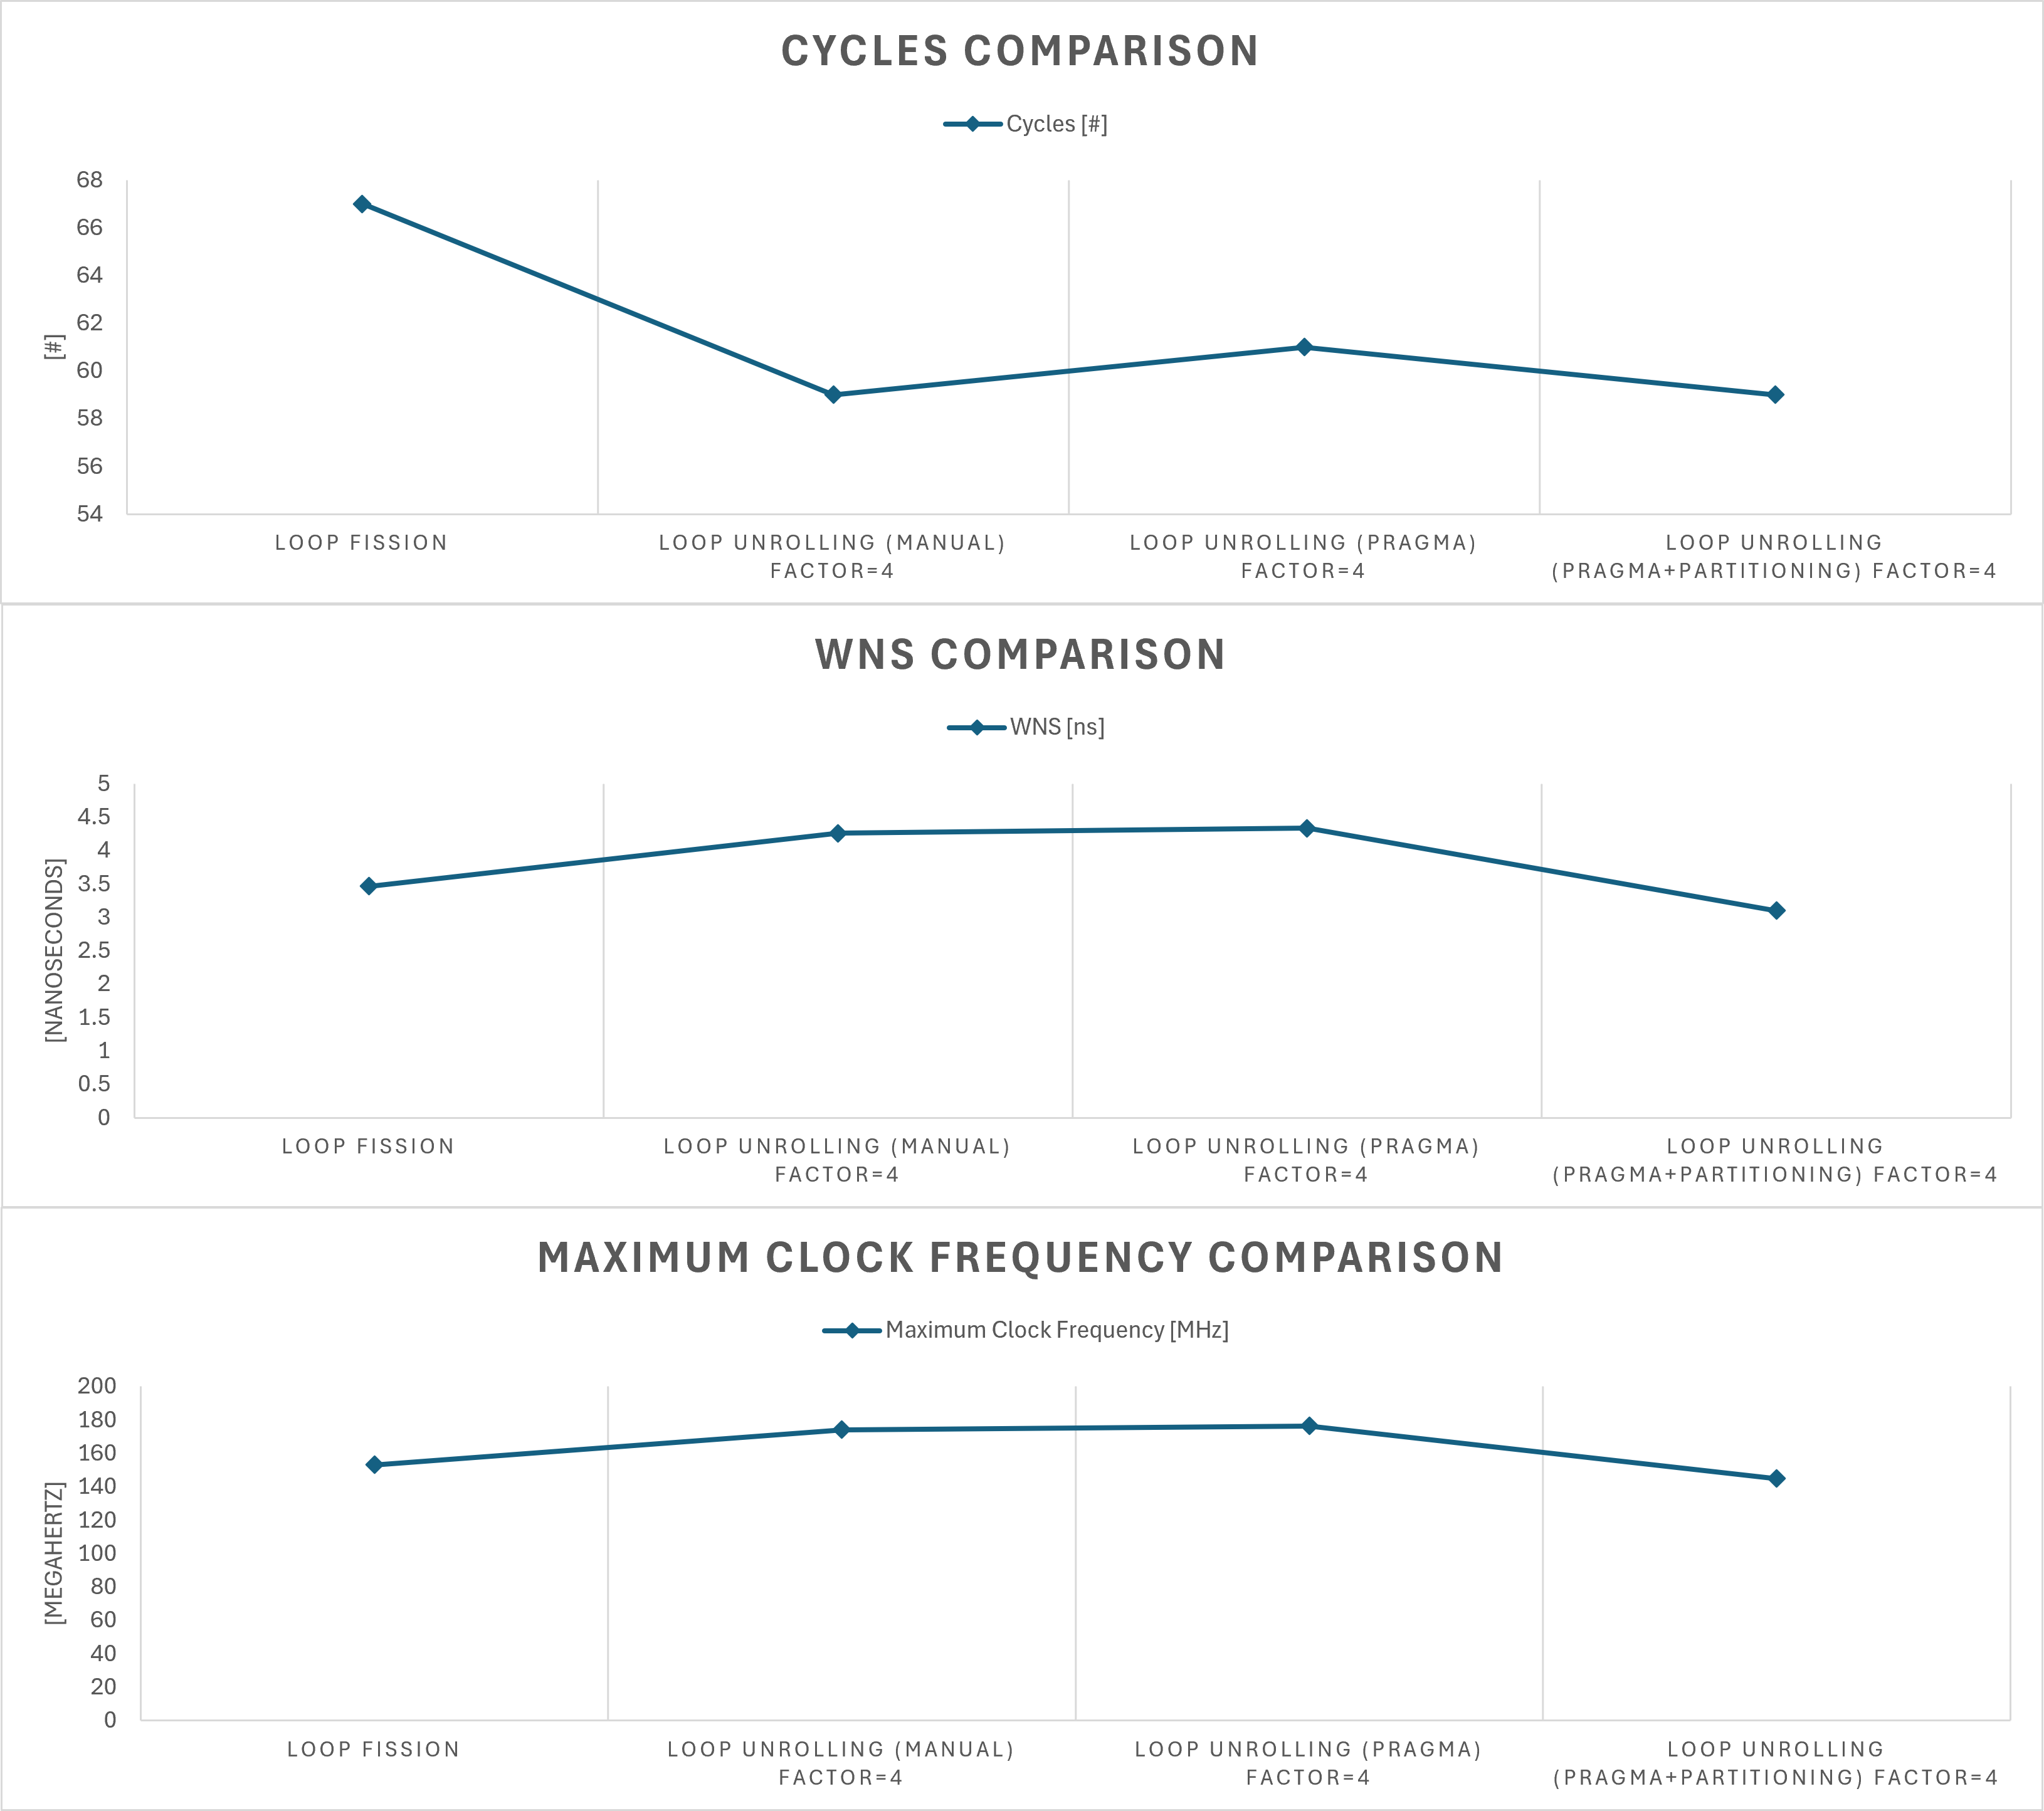
\includegraphics[width=0.8\textwidth]{solutions/loop_unrolling/factor4/loopunrollingfactor4timing.png}
    \caption{Vivado Loop Unrolling Factor=4 Timing Plot}
    \label{fig:vivado-loop-unrolling-factor4-solution-timing-plot}
\end{figure}

Analogamente all'unrolling di fattore pari a 2, anche in questo caso in corrispondenza della soluzione hardware basata su unrolling e partizionamento si ha un notevole aumento del contributo di potenza dinamica relativo al \textit{Clocks} comportando un aumento della potenza dinamica totale. 

\begin{table}[H]
    \centering
    \begin{tabular}{|c|c|c|c|c|c|c|c|}
        \hline
        \textbf{Solution} & \textbf{BRAM} & \textbf{Clock} & \textbf{Clocks} & \textbf{DSP} & \textbf{Logic} & \textbf{Set/}& \textbf{Data} \\
        & & \textbf{Enable} & & & & \textbf{Reset} & \\
        \hline
        Manuale & 1.32976193 & 0.382625905 & 0.253616716 & 0.921033497 & 0.543549308 & 0.010887122 & 0.585376518 \\
        \hline
        Automatico & 1.23103871 & 0.106978332 & 0.972227077 & 0.247065967 & 0.258892891 & 0.002585625 & 0.41881192 \\
        \hline
        Automatico & & & & & & & \\
        con & 0 & 0.328624592 & 2.560390625 & 0.298048515 & 1.146363211 & 0.0030065 & 1.324957004 \\
        Partitioning & & & & & & & \\
        \hline
    \end{tabular}
    \caption{Vivado Loop Unrolling Factor=4 Solution Dynamic Power Report [mW]}
    \label{tab:vivado-loop-unrolling-factor4-solution-dynamic-power-reproot}
\end{table}

\begin{table}[H]
    \centering
    \begin{minipage}[t]{0.45\linewidth}
        \centering
        \begin{tabular}{|c|c|}
            \hline
            \textbf{Solution} & \textbf{Dynamic Total} \\
            \hline
            Manuale & 4.026850996 \\
            \hline
            Automatico & 3.237600523 \\
            \hline
            Automatico & 5.661390447 \\
            con Partitioning & \\
            \hline
        \end{tabular}
        \caption{Vivado Loop Unrolling Factor=4 Solution Dynamic Power Report [mW]}
        \label{tab:vivado-loop-unrolling-factor4-solution-dynamic-power-reproot}
    \end{minipage}
    \hfill
    \centering
    \begin{minipage}[t]{0.45\linewidth}
        \centering
        \begin{tabular}{|c|c|}
            \hline
            \textbf{Solution} & \textbf{Energy Single Operation} \\
            \hline
            Manuale & 40.26850996 \\
            \hline
            Automatico & 32.37600523 \\
            \hline
            Automatico & 56.61390447 \\
            con Partitioning & \\
            \hline
        \end{tabular}
        \caption{Vivado Loop Unrolling Factor=4 Solution Energy Single Operation Report [pJ]}
        \label{tab:vivado-loop-unrolling-factor4-solution-solution-energy-single-operation-reproot}
    \end{minipage}
\end{table}

Bisogna notare un aspetto molto interessante. La potenza dinamica totale e l'energia per singola operazione associata alla soluzione hardware basata su loop unrolling automatico di fattore pari a 4 risultano essere pressocché le medesime di quelle relative all'unrolling automatico di fattore pari a 2. Questo potrebbe essere dovuto a ottimizzazione effettuate dal tool tramite la direttiva proprietaria dell'unrolling.
